\documentclass[10pt,a4paper]{article}
\usepackage[utf8]{inputenc}
\usepackage{amsmath}
\usepackage{amsfonts}
\usepackage{amssymb}
\usepackage{graphicx}
\usepackage[margin=0.6in]{geometry}
\begin{document}
\section*{\textit{Prüfungsrelevante} Verfahren, Sätze und Rechenregeln}
\section{Lineare Algebra}



\subsection{Komplexe Zahlen}
\begin{itemize}
\item $z=a+bi \in \mathbb{C}$ (\textbf{arithmetische} Darstellung)
\item $(\mathbb{C};+,\cdot)$ ist Körper der komplexen Zahlen (+ hat neutrales Element 0 und inverses Element $-z$; $\cdot$ hat neutrales Element 1 und inverses Element $z^{-1}$; beide assoziativ und kommutativ; $\cdot$ distributiv über +)
\item $\dfrac{z_{2}}{z}=\dfrac{z_{2}}{z}\cdot \dfrac{\overline{z}}{\overline{z}}=\dfrac{z_{2}\cdot \overline{z}}{a^2+b^2},\; \text{Re}(z)=a, \; \text{Im}(z)=b, \; \overline{z}=a-bi,\; r[\text{cos}(\varphi)+i\cdot \text{sin}(\varphi)]=re^{i\varphi}$
\item $r=\sqrt{a^2+b^2},\; \text{sin}(\varphi)=\dfrac{b}{r}, \;\text{cos}(\varphi)=\dfrac{a}{r}$; zur Bestimmung von $\varphi$ prüfen wo sin$^{-1}$ und cos$^{-1}$ den selben Wert annehmen 
\item \textbf{trigonometrische} und \textbf{eulersche} Darstellung erfolgt geometrisch in Polarkoordinaten $(r,\varphi)=(\vert z\vert,\text{arg}(z))$
\end{itemize}
\begin{center}
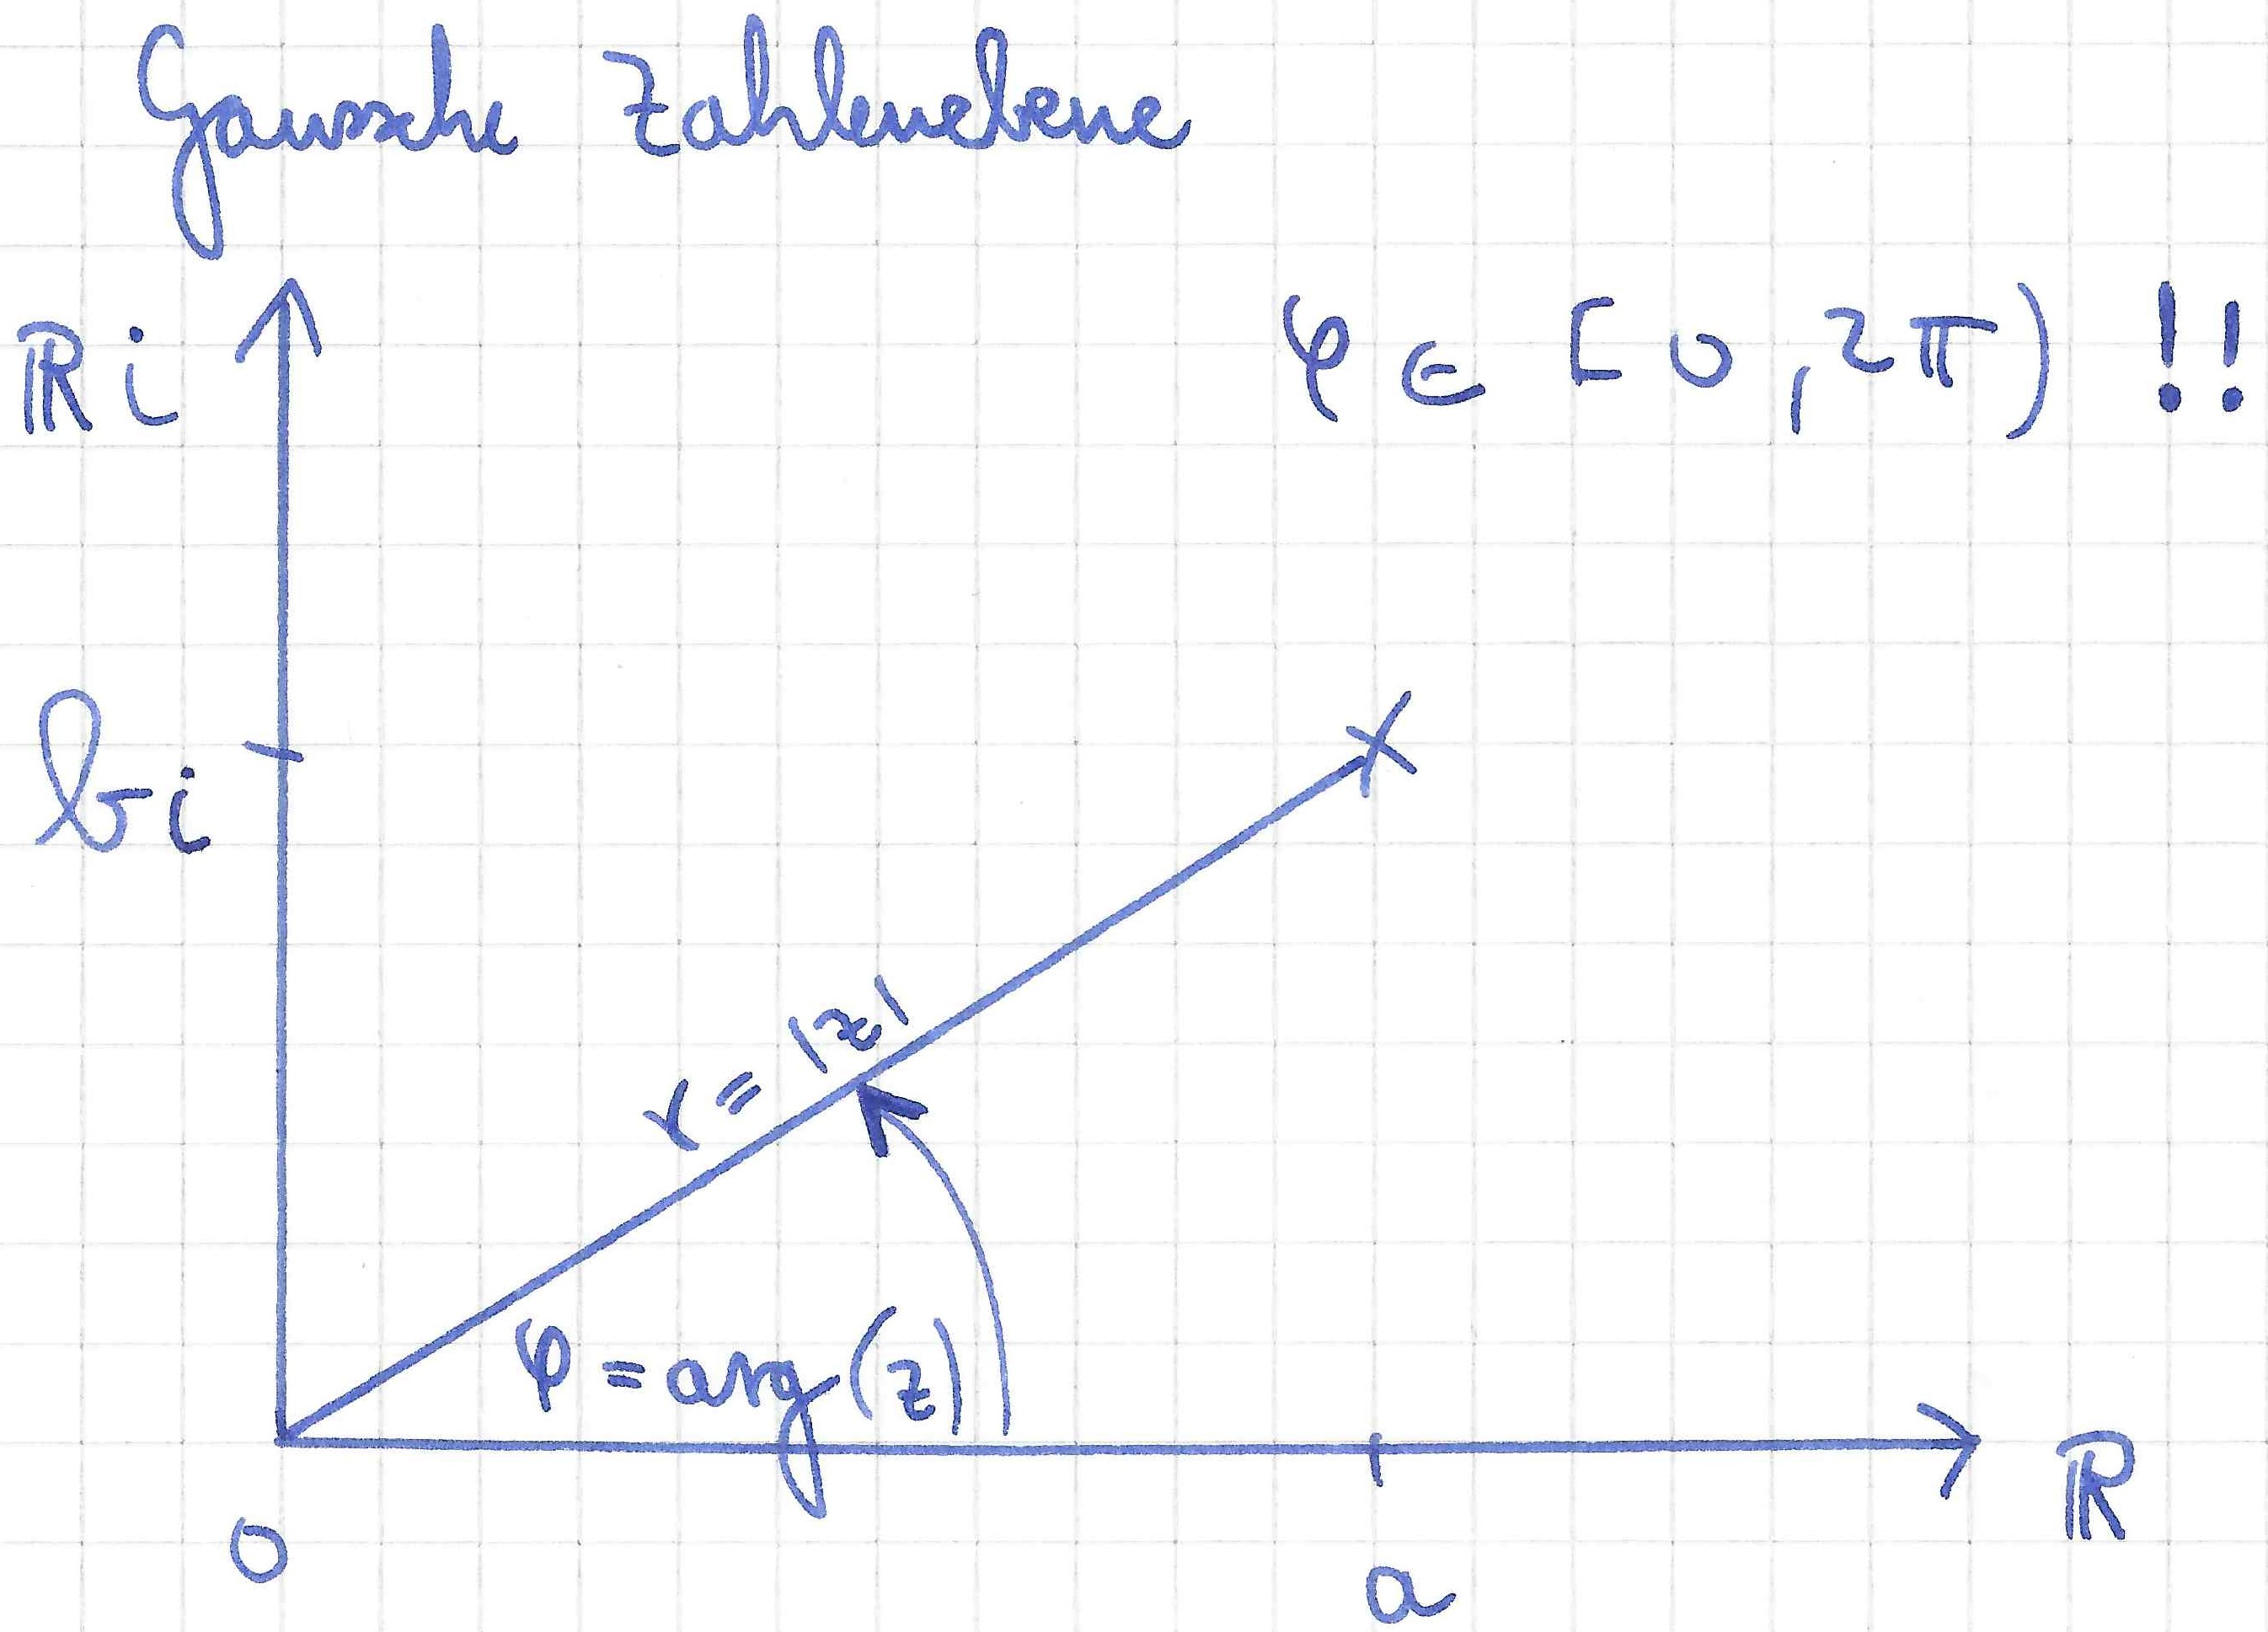
\includegraphics[scale=0.55]{gaussche_zahlenebene.jpg}\\
\textit{für komplexe Zahlen sind auch einfache Beweise prüfungsrelevant, rechnen mit euler/trig jedoch nicht}
\end{center}



\subsection{Rechnen mit Matrizen}
\begin{itemize}
\item Matrizen sind Abbildungen, die einem Paar $(i,j)$ ein Körperelement $a_{ij}$ zuordnen 
\item Matrix $A=(a_{ij})=(a_{ij})_{m \times n}$, es gibt $i$ horizontale Zeilen und $j$ vertikale Spalten; Hauptdiagonale von links oben nach rechts unten
\item spezielle Matrizen: Einheitsmatrix, Nullmatrix, quadratische Matrix (auch "n-reihig") und Diagonalmatrix (quadratisch und $a_{ij}=0$ für $i\neq j$)
\item Matrixmultiplikation: $(a_{ij})_{m\times n} \cdot (b_{ij})_{n \times p}=(\sum_{k=1}^{n} a_{ik}\cdot b_{kj})_{m \times p}$ 
\item $A^{T}$: Zeilen und Spalten vertauschen; $k(ABC)=AB(kC)=A(kB)C$ etc.
\item + kommutativ und assoziativ mit neutralem Element Nullmatrix; $\cdot$ assoziativ mit neutralem Element Einheitsmatrix und Nullmatrix absorbiert; $\cdot$ distributiv über + 
\item $(A+B)^{T}=A^{T}+B^{T},\; (kA)^{T}=kA^{T},\; (A^{T})^{T}=A,\; (A\cdot B)^{T}=B^{T}\cdot A^{T}$ (Reihenfolge !!)
\item $A^{-1}$ ist zu ermitteln durch $(A\mid E_{n})\rightsquigarrow (A \text{ in ZSF} \mid E_{n}') \rightsquigarrow (E_{n} \mid A^{-1})$ mit elementaren Zeilenumformungen\\ A in ZSF hat Nullzeilen $\Leftrightarrow \nexists A^{-1};\;\;\;$ Es gilt auch $A^{-1}=\text{det}(A)^{-1}(-1^{i+j}\text{ det}(A_{ji}))$
\item $(A\cdot B)^{-1}=B^{-1}\cdot A^{-1};\;\;A\in K^{2\times 2} \Rightarrow A^{-1}=\text{det}(A)^{-1}\cdot \begin{pmatrix} d& -b\\ -c&a\end{pmatrix}$
\end{itemize}



\subsection{LGS und Gauß-Jordan}
\begin{itemize}
\item GF2=$\left\lbrace 0,1\right\rbrace$, + und $\cdot$ für GF2 wie in $\mathbb{R}$ mod 2 ($\Rightarrow -a=a$)
\item \textbf{homogenes} LGS: alle Unveränderlichen sind 0, Nulltupel ist immer eine Lösung; \textbf{inhomogenes} LGS: mindestens eine Unveränderliche ist verscheiden von 0, Nulltupel keine Lösung  
\item Matrixschreibweise für LGS: $A\overrightarrow{x}=\overrightarrow{b}$, Kurzform: erweiterte Koeffizientenmatrix $(A \mid b)$
\item für LGS in \textbf{ZSF} (ZSF ist am besten am Beispiel zu verstehen, siehe Folie 3.7) gilt: $L=\emptyset \Leftrightarrow \exists b$ in einer Nullzeile das verschieden von 0 ist; umgekehrt für $L\neq \emptyset$ $\Rightarrow$ bei LGS mit Parameter ggf. Fallunterscheidung vornehmen!!
\item aus \textbf{reduzierter ZSF} (siehe Folie 3.9) kann man Lösung direkt ablesen; um (reduzierte) ZSF zu erhalten nutzt man \textbf{elementare Zeilenumformungen}: Zeilen vertauschen, Zeile mit $k\in K\setminus \left\lbrace 0\right\rbrace$ multiplizieren, $k$-faches einer Zeile zu anderer addieren
\item Gauss: LGS in ZSF, Lösbarkeitsentscheidung; Jordan: LGS in reduzierte ZSF
\item Nullzeilen dürfen bei Gauß-Jordan weggelassen werden (bei det nicht!), Spalten dürfen vertauscht werden (Variablennamen dranschreiben!)
\item notieren der Lösungsmenge z.B. als $L=\left\lbrace (2,3t,1,5k)\mid t,k \in K \right\rbrace$ oder als Menge von (hier 3) Vektoren, evtl. auch als Spanraum; so oder so Probe nicht vergessen!
\item GF2 LGS mit $n$ Parametern in der Lösungsmenge hat $2^{n}$ konkrete Lösungen ($\mathbb{C}/\mathbb{R}$ LGS unendlich viele)
\end{itemize}



\subsection{Vektorräume (VR)}
\begin{itemize}

%VR Axiome sollten nicht auswendig nötig sein

\item $K$-VR = algebraische Struktur $(V; \oplus , \underbrace{(k \mid k \in K)}_{\text{Skalarmultiplikation}})$ (beachte wo ; und wo , steht), muss VR-Axiome erfüllen
\item zu Unterscheiden sind $0_{V}$ und $0_{K}$, beide eindeutig bestimmt 
\item $kv=0_{V} \Leftrightarrow k=0_{K} \lor v=0_{V},\;\;\; (-k)v=\ominus kv, \;\;\; (-1)v=\ominus v\;\;\;\;$ (nach V5 ist $\ominus v$ Inverses von $v$)
\item $U$ heißt \textbf{Untervektorraum} (UVR) von $V$ wenn: 
\begin{enumerate} 
\item $0_{v} \in U$
\item $a,b\in U \Rightarrow a\oplus b \in U$ für alle $a,b \in U$ (abgeschlossen bzgl. $\oplus$)
\item $a\in U, k\in K \Rightarrow ka \in U$ für alle $a\in U,k\in K$ (abgeschlossen bzgl. $\odot$)
\item ($U\subseteq V$, immer zuerst prüfen!)
\end{enumerate}
\item $U_{1},U_{2}$ UVR von $V \Rightarrow U_{1} \cap U_{2}$ UVR von $V$; jeder UVR von $V$ ist ein $K$-VR
\end{itemize} 
\textit{VR Axiome nachweisen nicht prüfungsrelevant}



\subsection{Spannräume und Basen}
\begin{itemize}
\item für den $K$-VR $V$ mit $T\subseteq V$ ist Span$_{K}(T)=\langle T \rangle$ der kleinste UVR der $T$ enthält \item Berechnung: Span$(\left\lbrace v_{1},\dotsc ,v_{n}\right\rbrace)=\left\lbrace k_{1}v_{1}\oplus \dotsc \oplus k_{n}v_{n}\mid k_{1},\dotsc ,k_{n} \in K\right\rbrace $
\item $\langle V\rangle =V, \;\; \langle \emptyset \rangle =\left\lbrace 0_{v} \right\rbrace,\;\;$ für $T\subseteq V,V=$ Span$(T)$ ist $T$ \textbf{Erzeugendensystem} von $V$
\item Möglichkeiten zum Prüfen ob $T=\left\lbrace  v_{1}, \dotsc, v_{n} \right\rbrace$ z.B. Erzeugendensystem des $\mathbb{R}^{3}$ ist: 
\begin{enumerate}
\item gibt es überhaupt dim$(\mathbb{R}^3)=3$ lin. u. Vektoren in $T$?
\item ist LGS $\left(v_{1} \dotsc v_{n} \mid \begin{matrix} a\\  b\\c\end{matrix}\right)$ lösbar? 
\end{enumerate}
\item für eine \textbf{Basis} $B$ von $V$ gilt: $B$ ist lin. u. und $V=\text{Span}(B)$; alternativ kann geprüft werden: \begin{enumerate}
\item $B$ ist Erzeugendensystem von $V$, jede echte Teilmenge von $B$ ist kein Erzeugendensystem von $V$
\item $B$ ist lin. u., $B\cup \left\lbrace v \right\rbrace (v \in V,v\not\in B)$ ist lin. a. 
\item für $V$ mit dim$(V)=n$ genügt es zu Prüfen, ob ($B$ Erzeugendensystem mit $\vert B\vert=n$) oder ($B$ lin. u. und $\vert B\vert=n$)
\end{enumerate}
\item um Basis eines UVR $U=$ Span$(M)$ zu finden schreibe Vektoren in $M$ als LGS und bestimme damit größtmögliche lin. u. Teilmenge von $M$ 
\item zwei Basen von $V$ haben immer die gleiche Mächtigkeit $n=:\, $dim($V$); Basis vom Nullraum ist $\emptyset$
\item ist $B=(b_{1},\dotsc,b_{n})$ \underline{angeordnete} Basis von $V$, so lässt sich $v\in V$ als $v=k_{1}b_{1}\oplus\dotsc  \oplus k_{n}b_{n}$ darstellen und $v_{B}=\begin{pmatrix} k_{1}\\ \vdots\\ k_{n} \end{pmatrix}$ heißt \textbf{Koordinatenvektor} von $v$ bzgl. $B$ 
\end{itemize}



\subsection{Lineare Unabhängigkeit (lin. u. - keine offizielle Abkürzung)}
\begin{itemize}
\item $\left\lbrace v_{1}, \dotsc, v_{n} \right\rbrace$ ist lin. u. wenn gilt: $k_{1}v_{1} \oplus \dotsc \oplus k_{n}v_{n}=0_{V} \Rightarrow k_{1}=\dotsc=k_{n}=0_{K}$ 
\item in einer Menge lin. a. Vektoren kann \textit{mindestens ein} Vektor als LK der anderen dargestellt werden, es können aber i.A. \textit{nicht alle} Vektoren der Menge als LK der jeweils anderen dargestellt werden!
\item einige Möglichkeiten um $M=\left\lbrace v_{1}, \dotsc, v_{n}\right\rbrace$ auf lin. u. zu prüfen:
\begin{enumerate}
\item einfach LGS aufstellen (anders formuliert gilt also Ker$[(v_{1} \dotsc v_{n})]=\left\lbrace 0_{V} \right\rbrace \Rightarrow$ lin .u.)
\item es liegen in allen Vektoren in immer verschiedenen Komponenten Nullen vor $\Rightarrow$ lin. u.\\ (z.B. $\left\lbrace(0,1,0,4)^{T},(0,0,3,0)^{T},(2,0,0,0)\right\rbrace$ lin. u.) 
\item $0_{V} \in M \Rightarrow$ \textit{lin. a.}
\item  dim$(V)=n \Rightarrow$ mehr als $n$ Vektoren sind immer \textit{lin. a.}
\item rg$[(v_{1} \dotsc v_{n})]=n$ bzw. dim(Ker$[(v_{1} \dotsc v_{n})])=0$ bzw. det$[(v_{1} \dotsc v_{n})]\neq 0 \Rightarrow$ lin. u. 
\item $v_{1},\dotsc, v_{n}$ sind paarweise orthogonal $\Rightarrow$ lin. u.
\end{enumerate}

\end{itemize}
\textit{einfache Beweise sind prüfungsrelevant}



\subsection{Eigenschaften von Matrizen und LGS}
\begin{itemize}

%Begriff der affinen Teilräume hier erstmal ignoriert, spielt keine Rolle

\item \textbf{Kern} einer Matrix Ker$(A)$ ist Lösungsmenge von $(A\mid 0_{V})$ (dem zugehörigen homogenen LGS), Ker$(A)$ ist ein VR
\item Lösungsmengen inhomogener LGS sind keine VR; je zwei Lösungen des inhomogenen LGS unterscheiden sich um eine Lösung des homogenen LGS (=Kern der Koeffizientematrix)
\item für $A=(s_{1}\dotsc s_{n})$ ist der \textbf{Spaltenraum} Col$(A)=\text{Span}(\left\lbrace s_{1},\dotsc, s_{n}\right\rbrace)$, dim(Col$(A))$ heißt Spaltenrang (entspricht maximaler Menge lin. u. Spaltenvektoren von $A$); ganz analog für \textbf{Zeilenraum} Row$(A)$
\item Es gilt dim(Col$(A))$=dim(Row$(A))=:\text{rg}(A)\;\;\;$ (\textbf{Rang} von $A$); Berechnung: rg$(A)= \#$ nicht-Nullzeilen in ZSF
\item \textbf{Dimensionsformel: }$A\in K^{m \times n}\Rightarrow\text{rg}(A)+\text{dim(Ker}(A))=n$;  Lösbarkeitskriterium: $Ax=b$ lösbar $\Leftrightarrow \text{rg}(A)=\text{rg}(A \mid b)$
\item \# freie Parameter in der Lösungsmenge des homogenen LGS = dim(Ker$(A))=n-\text{ rg}(A)$
\end{itemize}
\textit{$\approx$ Ende LA 110.1}



\subsection{Lineare Abbildungen}
\begin{itemize}
\item sind $(V; \oplus_{V}, (k\mid k\in K)),(W; \oplus_{W}, (k\mid k\in K))$ VR über dem selben Körper, so ist $f:V \rightarrow W$ eine lineare Abbildung wenn für alle $a,b\in V,k\in K$ gilt:
\begin{enumerate}
\item $f(a \oplus_{V} b) =f(a)\oplus_{W} f(b)$
\item $f(ka)=kf(a)$
\item statt 1. und 2. kann auch $f(a\oplus_{V} kb)=f(a)\oplus_{W}kf(b)$
\end{enumerate}
\item $f(k_{1}v_{1}\oplus_{V}\dotsc \oplus_{V} k_{n}v_{n})=k_{1}f(v_{1})\oplus_{W}\dotsc\oplus_{W} k_{n}f(v_{n})$ 

% zeile 149 erstmal rauskommentiert weil ist eigentlich klar, und steht so ähnlich auch schon anderswo

\item Sei $\left\lbrace b_{1},\dotsc,b_{n}\right\rbrace$ Basis von $V.\;\;\;\;$   \textbf{f injektiv} $\Leftrightarrow \left\lbrace f(b_{1}), \dotsc,f(b_{n}) \right\rbrace $ lin. u. $\Leftrightarrow$ Ker$(f)=\left\lbrace 0_{V} \right\rbrace$\\
\textbf{f surjektiv} $\Leftrightarrow$ Span$(\left\lbrace f(b_{1}), \dotsc,f(b_{n}) \right\rbrace)=W\Leftrightarrow\text{Im}(f)=K$
\item\textbf{f bijektiv} $\Leftrightarrow \left\lbrace f(b_{1}), \dotsc,f(b_{n}\right\rbrace$ ist Basis von $W$\\ Für Beweise bzgl. dieser 3 Eigenschaften bieten sich oft Gegenbeispiele an!
\item Ker$(f)=\left\lbrace v \mid v \in V, f(v)=0_{W}\right\rbrace, 0_{V}\in\text{ Ker}(f);$ Im$(f)=\left\lbrace f(v) \mid v\in V\right\rbrace$, $0_{W}\in \text{Im}(f);$ beide UVR von $V$/$W$ 
\item \textbf{Dimensionsformel für lineare Abbildungen:} dim$(V)=n\Rightarrow\text{dim Im}(f)+\text{dim Ker}(f)=n$
\item $f(v)=f(k_{1}b_{1}+\dotsc + k_{n}b_{n})=k_{1}f(b_{1})+\dotsc k_{n}f(b_{n})$ ($f$ durch Bilder der Basisvektoren eindeutig bestimmt)
\item $\left\lbrace e_{1},\dotsc,e_{n}\right\rbrace$ Standardbasis von $K^{n},\;f: K^{n}\rightarrow K^{m}\Rightarrow f(v)=\underbrace{(f(e_{1})\dotsc f(e_{n}))}_{\text{Abbildungsmatrix A}}v$
\item allgemeiner gilt für $f:V\rightarrow W$ mit $B=(b_{1},\dotsc,b_{n})/C$ angeordnete Basis von $V/W$: $f(v)_{C}=A_{BC}\cdot v_{B}$ mit \textbf{darstellender Matrix} $A_{BC}=(f(b_{1})_{C}\dotsc f(b_{n})_{C});\;\;\Rightarrow\boldsymbol{f^{-1}:}\; A_{BC}^{-1}\cdot f(v)_{C}=v_{B} $ 
\item Aufstellen der darstellender Matrix: Setze $M_{B}=(b_{1} \dotsc b_{n})$, es gilt $M_{B}f(b_{i})_{B}=f(b_{i})\Rightarrow f(b_{i})_{B}= M_{B}^{-1}f(b_{i})\\ \Rightarrow A_{BB}=M_{B}^{-1}(f(b_{1})\dotsc f(b_{n}))\;\;\;\;$ (für $A_{BC}$ stattdessen $M_{C}^{-1}[f(b_{1})\dotsc f(b_{n})])$
%\item für $f_{1}:V_{1}\rightarrow V_{2},f_{2}:V_{2}\rightarrow V_{3}$ gilt $f_{2}\circ f_{1}$ hat darstellende Matrix $A_{B_{2}B_{3}}\cdot A_{B_{1}B_{2}}$
\item für $A_{BC}$ darstellende Matrix gilt Im$(f)=\text{Col}(A_{BC})$ und damit dim(Im$(f))=\text{ rg}(A_{BC})$; Ker$(f)=\text{Ker}(A_{BC})$
\end{itemize}
\textit{einfache Beweise sind prüfungsrelevant}


\newpage
\subsection{Determinante von $\boldsymbol{A\in K^{n\times n}}$}
\begin{itemize}
%\item det$(A)$ entspricht Faktor um den sich Flächeninhalt zwischen 2 Vektoren bei $f: x\mapsto Ax$ ändert ($A_{\text{P}}=ab\cdot \text{sin}\alpha)$ 
\item \textbf{Adjunkte} $A_{ij}$ entsteht aus $A$ durch streichen $i$-ter Zeile und $j$-ter Spalte 
\item Berechnung:
\begin{enumerate}
\item \textbf{Regel von Sarrus} für $A\in K^{3\times 3}:$ det$(A)=\underbrace{a_{11}a_{22}a_{33}}_{\text{Hauptdiagonale}}+\underbrace{a_{12}a_{23}a_{31}}_{\text{1 daneben}}+\underbrace{a_{13}a_{21}a_{32}}_{\dotsc}$\\
($a_{11}a_{22}-a_{12}a_{21}$ für $2\times 2)$
\hspace{2cm} $-\underbrace{a_{31}a_{22}a_{13}}_{\text{Nebendiagonale}}-a_{32}a_{23}a_{11}-a_{33}a_{21}a_{12}$
\item \textbf{Entwicklungssatz:} det$(a_{11})=a_{11}, \;\; \text{det}(A)=\underbrace{\sum_{i=1}^{n}}_{\text{bzw. }j}-1^{i+j}\cdot a_{ij}\cdot \text{det}(A_{ij})\;$ (Schachbrettregel für Vorzeichen, möglichst nach schwach besetzten Zeilen/Spalten entwickeln)
\item $A$ in die Form $\begin{pmatrix} a_{11} &&0\\ \vdots&\ddots&\\a_{n1}&\dotsc&a_{nn}\end{pmatrix}$ bringen (oder Dreieck andersherum) $\Rightarrow \text{det}(A)=a_{11}\cdot \dotsc \cdot a_{nn}$ 
\end{enumerate}
\item Umformungsregeln:
\begin{enumerate}
\item $\text{det}(B)=-\text{det}(A)$ wenn $B$ aus $A$ durch Vertauschen zweier Zeilen/Spalten entsteht
\item $\text{det}(B)=k\cdot \text{det}(A)$ wenn $B$ aus $A$ durch Multiplizieren von Zeile/Spalte mit $k\in K$ entsteht
\item det unverändert durch addieren von $k$-fachem einer Zeile/Spalte zu \textit{anderer} Zeile/Spalte
\end{enumerate}
\item $A$ enthält Nullzeile/Nullspalte/zwei paarweise lin. a. Zeilen/Spalten $\Rightarrow \text{det}(A)=0$
\item det$(A)=\det (A^{T});\;\;\det(A\cdot B)=\text{det(A)}\cdot \text{det}(B)$ (\textbf{Multiplikationssatz}) $\Rightarrow \text{det}(A^{-1})=\text{det}(A)^{-1}$
\end{itemize}



\subsection{Eigenwerte und Eigenvektoren (EW und EV)}
\begin{itemize}
\item $k\in K$ ist EW von $A$ wenn gilt $Av=kv$ ($\Rightarrow v$ ist EV zu $k$, dessen Richtung bei der von $A$ festgelegten linearen Abbildung nicht verändert wird), $v\in K^{n}\setminus \left\lbrace 0_{K^{n}}\right\rbrace$
\item Berechnung von $k$ über det$(A-kE_{n})=\chi_{A}(k)=0$, mit $\chi_{A}(k)$ als \textbf{charakteristisches Polynom;} Beachte beim Rechnen eventuelle Vielfachheiten der Nullstellen von $\chi$!!; Polynome mit deg$>2$ sollten mittels  Umformungsregeln für det vermieden werden, binomische Formeln ausnutzen, quadratische Ergänzung
\item da $\chi_{A}(k)=\det (A-kE_{n})$ gilt $\det(A)=\chi_{A}(0)$
\item Berechnung des \textbf{Eigenraums zum EW $\boldsymbol{k}$} ( d.h. dem UVR von $K^{n}$, der genau die EV zu k \textit{und} $0_{v}$ enthält): Eig$_{k}(A)=\text{Ker}(A-kE_{n})$
\item EV zu paarweise verschiedenen EW sind lin. u. (Beachte: durch Vielfachheiten können mehrere EV zu gleichen EW gehören, diese sind möglicherweise lin. a.)
\item $\det(A)=k_{1}\cdot \dotsc \cdot k_{n}$, $\text{ Spur}(A)=k_{1}+\dotsc +k_{n}$
\end{itemize}



\subsection{Eigenvektorbasen und diagonalisierbare Matrizen}
\begin{itemize}
\item Hat $K^{n}$ Basis die aus EV von $A\in K^{n\times n}$ besteht, so sprechen wir von einer Eigenvektorbasis bzgl. $A$ des $K^{n}$
\item $A$ mit EW $k_{1},\dotsc k_{n}$ und zugehörigen EV $v_{1},\dotsc,v_{n}$ ist diagonalisierbar g.d.w. gilt $\exists S,S^{-1}$ mit $S^{-1}\cdot A \cdot S =D$ und D Diagonalmatrix, es gilt:
\begin{itemize}
\item$S=(v_{1}\dotsc v_{n})$ und $ D=\begin{pmatrix}
k_{1}&&0\\&\ddots&\\0&&k_{n}
\end{pmatrix}$ (Reihenfolge der EV in $S$ = Reihenfolge der EW in $D$!!)
\end{itemize}
\item Äquivalente Aussagen:
\begin{enumerate}
\item A ist diagonalisierbar
\item $A$ hat $n$ lin. u. EV
\item $\exists$ Eigenvektorbasis bzgl $A$ des $K^{n}$
\end{enumerate}
\item \textbf{schnelles Potenzieren:} $A^{k}=(SDS^{-1})^{k}=SD^{k}S^{-1}$
\end{itemize}



\subsection{Skalarprodukt $\bullet$ und Orthogonalität in euklidischen $\mathbb{R}$-VR}
\begin{itemize}
\item für $u,v \in \mathbb{R}^{n}$ gilt $u\bullet v=u_{1}v_{1}+\dotsc +u_{n}v_{n}=u^{T}v$; für reelle Polynome ist $p(x)\bullet q(x)=\int_{\boldsymbol{-1}}^{\boldsymbol{1}} p(x)q(x) dx$
\item $\bullet$ ist \textbf{positiv definit} ($\geq 0$ für $u\bullet u$, 0 g.d.w. $u=0_{v}$), \textbf{bilinear} (distributiv über + von links und rechts; homogen von links und rechts), \textbf{symmetrisch}( =kommutativ)

%Eigenschaften Skalarprodukt möglicherweise nicht nötig aber da bin ich unsicher

\item ist $V$ ein $\mathbb{R}$-VR, so ist $(V;\bullet)$ ein euklidischer $\mathbb{R}$-VR, in dem gilt \textbf{Norm} $\Vert v \Vert=\sqrt{v\bullet v}$ 
\item cos$(\alpha)=\dfrac{u\bullet v}{\Vert u \Vert \cdot \Vert v\Vert}$ mit $\alpha\in [0,\pi]$!!$\;\;\;\; u \bullet v=0 \Leftrightarrow u\perp v$ $\;\;\;\;v$ ist \textbf{Einheitsvektor} wenn $\Vert v \Vert=v\bullet v=1$
\item es gilt S.d.P. und dessen Umkehrung: $\Vert u+v\Vert^2=\Vert u\Vert^2 +\Vert v \Vert^2 \Leftrightarrow u\perp v$

%Winkel und S.d.P evtl. auch nicht nötig

\item für $v\in V,u\in U=\text{Span}\left\lbrace b_{1},\dotsc,b_{n}\right\rbrace$ ist $U^{\perp}=\left\lbrace v\mid u\bullet v=0_{\mathbb{R}}\text{ für alle } u\in U\right\rbrace=\text{Ker}\begin{pmatrix}
b_{1}^{T}\\\vdots\\b_{n}^{T}
\end{pmatrix}$ \textbf{Orthogonalraum} von $U$ in $V$

%weitere Identitäten zu Orthogonalraum hier nicht enthalten da nicht gefordert; theoretisch wäre auch nichtmal Berechnung zum Verständnis nötig aber schadet vllt. auf den 2 A4 Seiten doch nicht...

\item orthogonale Projektion $\hat{v}$ von $v$ in $U=\text{Span}\left\lbrace b_{1},\dotsc,b_{n}\right\rbrace: \hat{v}=\text{proj}_{U}v=\dfrac{v\bullet b_{1}}{b_{1}\bullet b_{1}}b_{1}+\dotsc+\dfrac{v\bullet b_{n}}{b_{n}\bullet b_{n}}b_{n}$\\ 
(gilt nur für $\left\lbrace b_{1},\dotsc,b_{n}\right\rbrace$ OGB, sonst erst Gram-Schmidt anwenden!!) 
\item \textbf{Satz über die Orthogonalzerlegung:} für $v\in \mathbb{R}$-VR $R$,$U$ UVR von $R$ gilt: $v=\hat{v}+w$ mit $\hat{v}\in U$ und $w\in U^{\perp}$
\end{itemize}



\subsection{Orthogonal- und Orthonormalbasen (OGB/ONB -keine offiziellen Abkürzungen), Gram-Schmidt-Verfahren }
\begin{itemize}
\item OGB ist Basis mit paarweise orthogonalen Basisvektoren, ONB ist OGB mit normierten Basisvektoren\\
(Berechnung des normierten Vektors: $v'=\dfrac{v}{\Vert v\Vert}$)
\item ist $\left\lbrace b_{1},\dotsc, b_{n}\right\rbrace$ OGB von $V$ und $v\in V$ dann gilt $v=\text{proj}_{V}v$
\item Konstuktion einer OGB $\left\lbrace b_{1},\dotsc, b_{n}\right\rbrace$ von UVR $U$ eines $\mathbb{R}$-VR (geg.: Basis $\left\lbrace u_{1} \dotsc u_{n}\right\rbrace$):
\begin{enumerate}
\item $b_{1}:=u_{1}$
\item $b_{i+1}:=u_{i+1}-\text{proj}_{\text{Span}(\left\lbrace b_{1},\dotsc,b_{i}\right\rbrace)}u_{i+1}$
\end{enumerate}
\item ist $u_{i}$ fälschlicherweise lin. a. von den bereits behandelten Vektoren, so wird $b_{i}=0_{\mathbb{R}^{n}}$
\end{itemize}



\subsection{Äquivalente Aussagen für $\boldsymbol{A\in K^{n\times n}}$}
\begin{itemize}
\item Spaltenvektoren von $A$ sind lin. u. 
\item Zeilenvektoren von $A$ sind lin. u.
\item $A$ in ZSF hat keine Nullzeilen 
\item $\text{rg}(A)= n $
\item $\text{Ker}(A)=\left\lbrace 0_{K^{n}}\right\rbrace$
\item $\text{dim Ker}(A)=0$
\item $\text{det}(A)\neq 0$
\item $\exists A^{-1}$ 
\item $\exists (A^{T})^{-1}$
\item durch $A$ definierte lineare Abbildung bijektiv
\end{itemize}
\noindent \textit{Bezeichnungen die nicht in der Aufgabenstellung gegeben sind müssen ggf. selber gesetzt werden, es kann z.B. für eine Menge von Vektoren nötig sein erst $b_{1}:=\dotsc$ etc. zu setzen}
\end{document}